\documentclass{article}
\usepackage[a3paper,landscape,bindingoffset=0in,left=0.5in,right=0.5in,top=1in,bottom=1in,footskip=.25in]{geometry}
\usepackage{multicol}
\usepackage{multirow}
\usepackage{graphicx}
\usepackage{tabularx}
\usepackage{showframe} % show frame margin
\usepackage{blindtext}

\setlength{\leftmargin}{0cm}
\setlength{\marginparwidth}{0cm}
\setlength{\columnsep}{1cm}
\pagenumbering{gobble}

\title{OLL and PLL Algorithms}
\author{Dir Sulaiman}


\begin{document}
    \begin{multicols}{2}

        \section*{Corner Permutations Only}
        \begin{tabular}{|c|c|c|c|l}
            \centering
            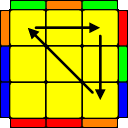
\includegraphics[width=0.03\textwidth]{images/pll/aa.jpg} & UPUPEKLDL LUL & 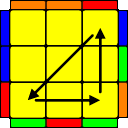
\includegraphics[width=0.03\textwidth]{images/pll/ab.jpg} & UPISSWLS\\
            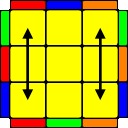
\includegraphics[width=0.03\textwidth]{images/pll/e.jpg} & UPUPEKLDL & \includegraphics[width=0.03\textwidth]{images/pll/solved.jpg} &  \\
        \end{tabular}

        \section*{Edge Permutations Only}
        \begin{tabular}{|c|ll|c|l} %pakai @{} untuk hilangkan spasi dengan garis
            \centering
            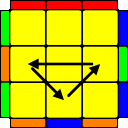
\includegraphics[width=0.03\textwidth]{images/pll/ua.jpg} & UPUPEKLDL LUL & 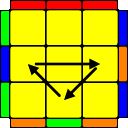
\includegraphics[width=0.03\textwidth]{images/pll/ub.jpg} & UPISSWLS\\
            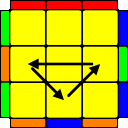
\includegraphics[width=0.03\textwidth]{images/pll/ua.jpg} & UPUPEKLDL & 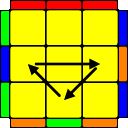
\includegraphics[width=0.03\textwidth]{images/pll/ub.jpg} & UPISSWLS\\
            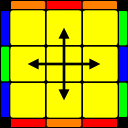
\includegraphics[width=0.03\textwidth]{images/pll/h.jpg} & UPUPEKLDL & 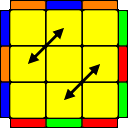
\includegraphics[width=0.03\textwidth]{images/pll/z.jpg} & UPISSWLS\\
        \end{tabular}

        \section*{Adjacent Corner Swap}
        \begin{tabular}{|c|ll|c|l} %pakai @{} untuk hilangkan spasi dengan garis
            \centering
            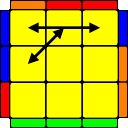
\includegraphics[width=0.03\textwidth]{images/pll/ja.jpg} & UPUPEKLDL LUL & 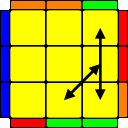
\includegraphics[width=0.03\textwidth]{images/pll/jb.jpg} & UPISSWLS\\
            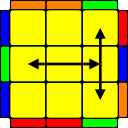
\includegraphics[width=0.03\textwidth]{images/pll/t.jpg} & UPUPEKLDL & 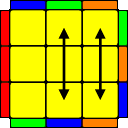
\includegraphics[width=0.03\textwidth]{images/pll/f.jpg} & UPISSWLS\\
            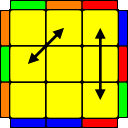
\includegraphics[width=0.03\textwidth]{images/pll/ra.jpg} & UPUPEKLDL & 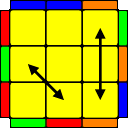
\includegraphics[width=0.03\textwidth]{images/pll/rb.jpg} & UPISSWLS\\
        \end{tabular}

        \section*{Diagonal Corner Swap}
        \begin{tabular}{|c|ll|c|l} %pakai @{} untuk hilangkan spasi dengan garis
            \centering
            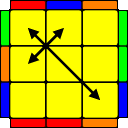
\includegraphics[width=0.03\textwidth]{images/pll/y.jpg} & UPUPEKLDL LUL & 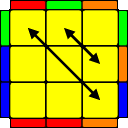
\includegraphics[width=0.03\textwidth]{images/pll/v.jpg} & UPISSWLS\\
            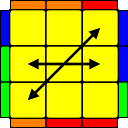
\includegraphics[width=0.03\textwidth]{images/pll/na.jpg} & UPUPEKLDL & 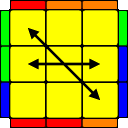
\includegraphics[width=0.03\textwidth]{images/pll/nb.jpg} & UPISSWLS\\
        \end{tabular}

        \section*{G Permutations}
        \begin{tabular}{|c|ll|c|l} %pakai @{} untuk hilangkan spasi dengan garis
            \centering
            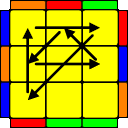
\includegraphics[width=0.03\textwidth]{images/pll/ga.jpg} & UPUPEKLDL LUL & 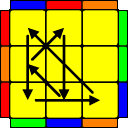
\includegraphics[width=0.03\textwidth]{images/pll/gb.jpg} & UPISSWLS\\
            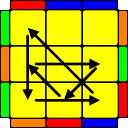
\includegraphics[width=0.03\textwidth]{images/pll/gc.jpg} & UPUPEKLDL & 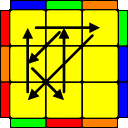
\includegraphics[width=0.03\textwidth]{images/pll/gd.jpg} & UPISSWLS\\
        \end{tabular}


        \columnbreak

        \begin{tabular}{ccc}
            \hline
            \multicolumn{2}{c}{\multirow{2}{*}{Multi-col-row}}&X\\
            \multicolumn{2}{c}{}&X\\
            \hline
            X&X&X\\
            \hline
        \end{tabular}


        \blindtext[2]

    \end{multicols}
\end{document}
